\def \M{\mathcal{M}}
\newcommand{\prob}{{\rm Prob~}}
\chapter{Theoretical consideration}
\myabstract{A short overview of the math that is used by the program \migrate. If you want to treat \migrate as a black box, then skip this section.}
The program \migrate infers population genetic parameters from genetic data. Essentially we want to find the parameters and their probability distribution given the Data
\begin{align}
   \prob(\P | \Dd). \notag
\end{align} 

This probability of the population genetics parameters $\P$, 
such as population sizes or migration rates, can be calculated in principle by integrating over all possible 
relationships 
$\G$ 
of the sample data 
$\Dd$ 
using   an expansion of the coalescent theory \citep{kingman1982-27,kingman1982-235,kingman2000-1461} which
includes migration \citep{hudson1991-1,nath1993-841,notohara1990-59}.
\begin{align}
\prob(\P | \Dd) &=  \frac{\prob( \P, \Dd)}{\prob(\Dd)} \\
\prob(\P | \Dd) &=  \frac{\prob(\P) \prob( \Dd | \P)}{\prob(\Dd)}\\
\intertext{A Bayesian would tell us to use this}
\label{BAYES}
\prob(\P | \Dd) &=  \frac{\prob(\P) \int_G \prob(G | \P) \prob( \Dd | G)dG}{\prob(\Dd)}  \\ 
\intertext{whereas as likelihoodist would suggest to use this}
\label{LIKELIHOOD}  
{\rm L}(\P) = \prob(\Dd | \P) &=   \int_G \prob(G | \P) \prob( \Dd | G)dG.   
\end{align}
 
 The integration over all genealogies is not a simple integral, but a sum over all possible labeled histories and integrals over all possible branch lengths $b_i$
\begin{align}
{\rm L}(\P) &= \sum_T \int_{b_1} ... \int_{b_k} \prob(T,\underline{b} | \Theta) \prob(\Dd | T,\underline{b}) db_1...db_k.
\end{align}
\migrate can use both approaches to estimate the parameters, the likelihood approach is more mature (because I started coding with that) than the Bayesian approach, although, currently I favor the Bayesian implementation over the ML implementation in \migrate.
Specifically, \migrate estimates migration rates and effective population sizes of 1 to many populations
using genetic data (Fig 1).  The parameters to estimate are
\begin{align}
\label{PARAMETERS}
\P &= \left(\begin{matrix}  \underline{\Theta} & \underline{\M} \end{matrix}\right)  \\
\intertext{with mutation-scaled population sizes}
\underline{\Theta} &= \left( \begin{matrix} \Theta_1 & \Theta_2 & ... & \Theta_n \end{matrix} \right) \\
\intertext{and mutation-scaled immigration rates}
\underline{\M} &= \left( \begin{matrix} - & \M_{2 \rightarrow 1} & \M_{3 \rightarrow 1} & ... & \M_{n \rightarrow 1} \\  \M_{1 \rightarrow 2} & - & \M_{3 \rightarrow 2} & ... & \M_{n \rightarrow 2}\\ 
... & ... & ... & ... & ... \\
\M_{1 \rightarrow n}  & ... & ... & \M_{(n-1) \rightarrow n}  & - \end{matrix} \right)
\end{align}

with mutation-scaled effective population size $\Theta_i$ which is $x \times$ effective population size $\times$ mutation rate per site per generation $\mu$, $x$ is a multiplier that depends on the ploidy and inheritance of the data, for nuclear data it $x=4$, for haploid data its $x=2$, and for mtDNA in vertebrates with female-only transition it is $x=1$. Life history is important, for example fish like Grouper change sex in their lifetime and therefore all individuals can transmit mtDNA resulting in having $x\simeq2$ and not $x=1$. The mutation-scaled effective immigration rate $\M$ is the immigration rate $m$ divided by the mutation rate $\mu$, it is a measure of how much more important immigration is over mutation to bring new variants into the population. If $\Theta$ and $\M$ are multiplied together the number of immigrants per generation $xNm$ can b e calculated.

\begin{figure}[htb]
\begin{center}
\leavevmode
\hbox{%
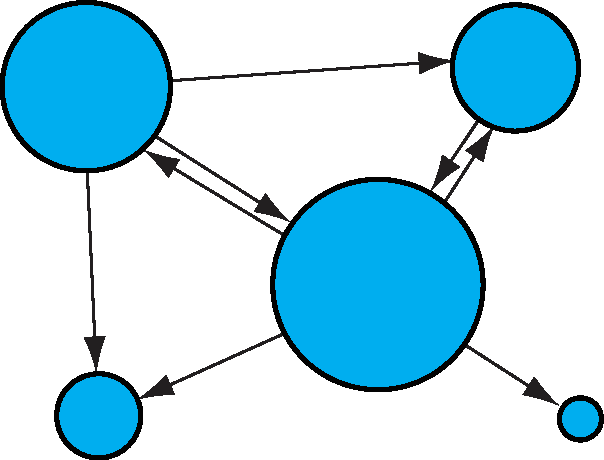
\includegraphics[scale=0.6]{mim/example-migration-lightblue}}
\end{center}
\begin{picture}(0,0)(0,0)
\put(76,50){$M_{14}$}%
\put(75,40){$M_{12}$}%
\put(52,26){$M_{13}$}%
\put(103,20){$M_{15}$}%
\put(89,42){$M_{42}$}%
\put(70,22){$M_{23}$}%
\put(67,32){$M_{21}$}%
\put(102,36){$M_{24}$}%
%
\put(59,45){$\Theta_1$}
\put(89,25){$\Theta_2$}
\put(52,14){$\Theta_3$}
\put(103,48){$\Theta_4$}
\put(115,13){$\Theta_5$}
\end{picture}

\caption{Populations exchanging migrants with rate $m_{j \rightarrow i}$ per generations and with size 
$N_e$. The parameters are scaled by mutation rate $\mu$ which is with sequence data per site per generation. The estimated parameters are therefore: $\Theta_i$ which is $x N^{(i)}_e \mu$ and 
$\M_i$ 
which is $m_i/\mu$, the migration estimate is often also expressed as $xNm$ which is just $\Theta \M$, x is the inheritance parameter and depends on the data, commonly 4 for nuclear data, and 1 for mtDNA data. The example model is not a complete (full) model because some migration routes are not estimated and set to zero.}
\label{FIG1}
\end{figure}


\section{Maximum likelihood estimation of migration rates}
The estimates of the parameters $\P$ are found by maximizing formula (\ref{LIKELIHOOD}.)
Unfortunately, this integral cannot be calculated by an analytical or simple numerical approach. This problem is solved by using a Markov chain Monte Carlo approach with importance
sampling first described by \cite{Metropolis:1953:ESC} and refined by \cite{hastings1970-97}. For an introduction see \cite{Hammersley:1964:MCM}or \cite{chib:1995:umh}, 
and see \cite{kuhner1995-1421} for a first application using MCMC in the context of coalescence theory.
We bias the search path through all trees towards trees with higher likelihoods (Fig. 2)
and have then to correct for this. The likelihood formula changes to
\begin{align}
\frac{L(\P)}{L(\P_0)} &= \frac{1}{m}\sum_i^m\ \frac{ \prob(D\ |\ g_i)\ \prob( g_i\ |\ \P)}
{\prob(D\ |\ g_i)\ \prob( g_i\ |\ \P_0)}.
\end{align}
Such an approach is reasonable because summands with low probabilities
will contribute very little to the final likelihood. For more information on the base model, you should read \cite{beerli:1999:mle} and \cite{kuhner1995-1421}.

The approximation of the likelihood using a ratio makes it difficult to
compare different runs of the program. The program reports a likelihood
that is actually a ratio of likelihoods and since we recalculate the
parameters for each chain, the values for $\P_0$ are different
between runs, and therefore it is impossible to compare them. A comparison of the parameters, of course, is still possible.
An escape of this 
problem is to run the program using the full model (e.g. $n \times n$ parameters and use the likelihood ratio test for specific scenarios.

\begin{figure}[hbt]
\begin{center}
\leavevmode
\hbox{%
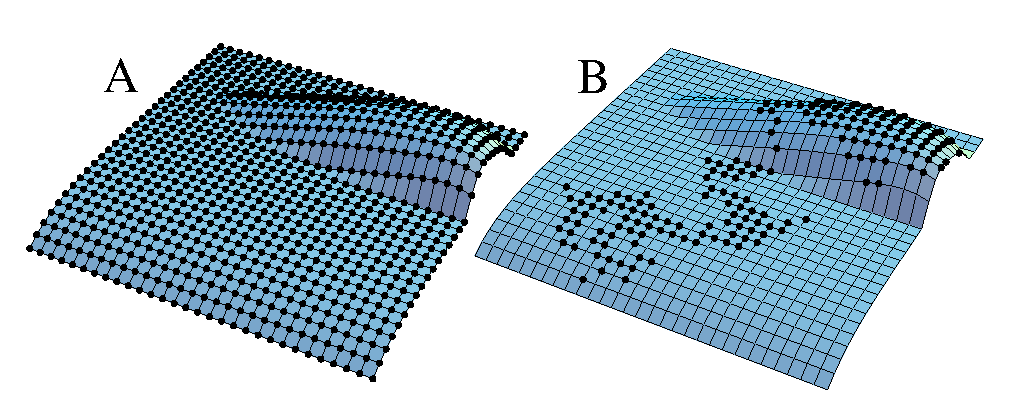
\includegraphics[scale=0.8]{mim/planes_orig}}
\end{center}
\caption{
(A) On an imaginary, infinite likelihood surface  we would need to sample every possible
genealogy and sum all these values which is not possible, but trees with low probability will not contribute much to the final likelihood,  (B) by biasing towards better trees we can sample effectively from those trees with high 
contribution to the final likelihood and can approximate the likelihood.
}
\label{FIG2}
\end{figure}
\vskip 1cm
\section{Bayesian inference}
\migrate allows to estimate the parameters using a Bayesian paradigm (see formula \ref{BAYES}) instead of the likelihood framework, simulation studies show that there are few differences with the ML runs, although some combinations of parameters might be be easier to estimate with the Bayesian approach \citep{beerli:2006:CBM}. Since in a Bayesian inference the driving parameters are changing often, this type of analysis might get better results on genealogy and parameter landscapes that are very choppy with many high peaks (see Fig. 2 for an example with a smooth surface). \migrate allows to use several different prior distributions. The parameter $r$ is the a uniform random number from (0,1].

\subsection{Prior distributions}
\vskip -0.5cm
\subsubsection{Uniform prior distribution}
The parameters have a uniform distribution between a minimal and a maximal value of the parameters, there is a set of minima and maxima for $\underline{\Theta}$ and $\underline{\M}$.
\migrate calculates the uniform by using
\begin{gather}
\label{UNIPRIOR}
    \prob(\P_i) =  \frac{1}{\P_{max} - \P_{min}} \\
    \intertext{it is implemented using a windowing method with window size $\Delta$, that is preferrably around 1/10 of the whole range.}
    \P_{\rm new} =  \P_{\rm old} + (2 \Delta r - 1) \begin{cases} \P_{\rm new} < \P_{\rm min}  &  \P_{\rm min} + |\P_{\rm min} - \P_{\rm new}| \\
     \P_{\rm new} > \P_{\rm max}  &  \P_{\rm max} - |\P_{\rm max} - \P_{\rm new}| \end{cases}
\end{gather}

\subsubsection{Exponential prior distribution}
The parameters have a exponential distribution, \migrate calculates three versions\\
\textsl{Simple exponential prior distribution}
\begin{align}
\label{EXPPRIOR}
    \prob(\P_i) &=  \int_0^\infty exp( -P_{i} / P_{\rm mean}) / P_{\rm mean} d\P_i = exp(- P_{i}/P_{\rm mean}) \\
    \P_{\rm new} &=  - \P_{\rm mean}\ ln(r)
\end{align}
\textsl{Exponential prior distribution with fixed window}
\begin{align}
\label{WEXPPRIOR}
    \prob(\P_i, \P_{\rm min}, \P_{\rm max}) &=  \frac{\int_{\P_{\rm min}}^{\P_{\rm max}} exp( -P_{i} / P_{\rm mean}) / P_{\rm mean} d\P_i}{exp(-P_{\rm min}/P_{\rm mean}) - exp(-P_{\rm max}/P_{\rm mean})}\\ 
     &= \frac{exp(-P_{\rm min}/P_{\rm mean}) - exp(-P_{\rm x}/P_{\rm mean})}{exp(-P_{\rm min}/P_{\rm mean}) - exp(-P_{\rm max}/P_{\rm mean})} \\
    \P_{\rm new} &=  - \P_{\rm mean}\ ln(\frac{r}{exp(\P_{\rm max}/\P_{\rm mean})}-\frac{r-1}{exp(\P_{\rm min}/\P_{\rm mean})}); 
\end{align}
\textsl{Exponential prior distribution with variable window}
\begin{align}
\label{AEXPPRIOR}
    \prob(\P_i | \P'_i,  \P_{\rm min}, \P_{\rm max}) &=  \frac{2 \int_{\P'_i - \Delta}^{\P'_i + \Delta} exp( -P_{i} / P'_i) / P'_i d\P_i}{exp(1) Csch(\Delta / P'_i)}\\ 
     &= \frac{(exp(\Delta + P_i)/P'_i - exp(1)) Csch(\Delta/\P'_i)}{2 exp(\P_i/\P'_i)} 
     \end{align}
     \begin{align}
    \P_{\rm new} &=  \P'_i - \P'_i ln(exp(\Delta/\P'_i) - 2 r Sinh(\Delta / \P'_i))\begin{cases} \P_{\rm new} < \P_{\rm min}  &  \P_{\rm min} + |\P_{\rm min} - \P_{\rm new}| \\
     \P_{\rm new} > \P_{\rm max}  &  \P_{\rm max} - |\P_{\rm max} - \P_{\rm new}| \end{cases}
\end{align}
